\documentclass[12pt,a4paper]{article}
\usepackage[T2A]{fontenc}
\usepackage[utf8]{inputenc}
\usepackage[russian]{babel}
\usepackage[margin=2cm]{geometry}
\usepackage{amsmath}
\usepackage{graphicx}
\usepackage{tikz}
\usetikzlibrary{arrows.meta,positioning}
\usepackage{fancyvrb}
\usepackage{hyperref}
\hypersetup{hidelinks}
\setlength{\parindent}{1.25cm}
\setlength{\parskip}{0.25em}
\sloppy
\begin{document}
\begin{titlepage}
\begin{center}
[Название вуза]\\[0.5cm]
[Факультет и кафедра]\\[3cm]
{\Large Отчёт по лабораторной работе 2}\\[0.5cm]
{\large Модули и пакеты Python}\\
{\large Объектно ориентированное программирование}\\[1cm]
Калькулятор рецептов\\[0.4cm]
Вариант 9 по порядку\\
Строка с меткой 11 в методических указаниях\\
Уровень Well-done
\end{center}
\vfill
\begin{flushright}
Выполнил(а): [ФИО]\\
Группа: [вписать]\\[0.5cm]
Проверил(а): [ФИО преподавателя]
\end{flushright}
\vfill
\begin{center}
[Город], 2026
\end{center}
\end{titlepage}
\tableofcontents
\newpage

\section{Цель и условие работы}
Разработать MVP на Python с модульной структурой и объектно ориентированной моделью.
Применить абстрактные классы, наследование, свойства, специальные методы,
автоматическое тестирование, сохранение результатов и упаковку в Docker.

Девятое задание по порядку --- <<Рецепты>>. В таблице после номера 7 сразу идёт 10;
поэтому девятая строка имеет напечатанную метку 11.
Объекты: вок, бургер, пицца. Задача: расчёт энергетической ценности и стоимости
рецепта по используемым ингредиентам.

Реализованы единый консольный интерфейс для Windows и Docker,
пакет из трёх рабочих модулей, Excel-отчёт,
README и зависимости. Для Medium добавлены ABC, абстрактное свойство,
наследование, управляемые атрибуты, специальные методы и pytest.
Для Well-done добавлены SQLite и Dockerfile с установкой библиотек при сборке.

\section{Репозиторий}
Ссылка на репозиторий с программной реализацией: \url{https://github.com/stitch2277-bit/lab_2_a}.

\section{Математическая модель}
Для ингредиента $i$ вводятся масса $m_i$ в граммах, калорийность $k_i$ в ккал
на 100 г и цена $p_i$ в рублях на 100 г:
\[
 E_i=\frac{m_i k_i}{100},\qquad
 C_i=\frac{m_i p_i}{100}.
\]
Общая масса, калории и стоимость:
\[
 M=\sum_i m_i,\qquad E=\sum_i E_i,\qquad C=\sum_i C_i.
\]
Для $n$ одинаковых порций и базы 100 г:
\[
 M_{\text{порции}}=\frac{M}{n},\quad
 E_{\text{порции}}=\frac{E}{n},\quad
 C_{\text{порции}}=\frac{C}{n},\quad
 E_{100\text{ г}}=\frac{100E}{M}.
\]

Масса каждого ингредиента положительна, поэтому $M>0$. Число порций ---
положительное целое. Цена и калорийность неотрицательны.
Вычисления выполняются с Decimal, показ --- с округлением до двух знаков
по правилу ROUND\_HALF\_UP. Слагаемые до суммирования не округляются.

Масса готового блюда принимается равной сумме масс ингредиентов.
Не учитываются потери при готовке, закупка целых упаковок, электричество,
доставка, работа повара и наценка. Продукты и цены примеров условные;
пользователь вводит нужные значения с упаковки.

\section{Структура и классы}
Основная программа \texttt{main.py} без аргументов открывает консольное меню.
Локальный батник и Docker запускают этот же файл. Он подключает пакет \texttt{recipes}:
\begin{itemize}
\item \texttt{models.py} --- классы предметной области, проверки и формулы;
\item \texttt{storage.py} --- класс CalculationStore для SQLite;
\item \texttt{reports.py} --- текстовый результат и настоящий Excel 97--2003 .xls.
\end{itemize}
Файл \texttt{\_\_init\_\_.py} обозначает пакет и не содержит рабочей логики.

\subsection{UML схема}
\begin{figure}[htbp]
\centering
\begin{tikzpicture}[
  box/.style={draw,align=left,text width=5.7cm,font=\small,inner sep=6pt},
  smallbox/.style={draw,align=center,text width=2.1cm,font=\small,inner sep=6pt},
  inheritance/.style={-{Triangle[open,length=3mm]},thick}
]
\node[box] (recipe) {Recipe \textit{(abstract)}\\
\rule{5.7cm}{0.2pt}\\
name, portions, ingredients\\
kind \textit{(abstract property)}\\
total\_grams, total\_calories, total\_cost\\
\rule{5.7cm}{0.2pt}\\
snapshot(), \_\_init\_\_(), \_\_str\_\_(), \_\_len\_\_()};
\node[box,right=0.9cm of recipe] (ingredient) {Ingredient\\
\rule{5.7cm}{0.2pt}\\
name, grams, kcal\_per\_100g\\
price\_per\_100g, calories, cost\\
\rule{5.7cm}{0.2pt}\\
\_\_init\_\_(), \_\_str\_\_(), \_\_repr\_\_()};
\node[smallbox,below=1.4cm of recipe.south west,anchor=north west] (wok) {Wok};
\node[smallbox,right=0.3cm of wok] (burger) {Burger};
\node[smallbox,right=0.3cm of burger] (pizza) {Pizza};
\draw[inheritance] (wok.north) -- (recipe.south);
\draw[inheritance] (burger.north) -- (recipe.south);
\draw[inheritance] (pizza.north) -- (recipe.south);
\draw[{-Diamond[open,length=3mm]}] (ingredient.west) -- node[above,font=\scriptsize] {1..1000} (recipe.east);
\node[box,below=1.4cm of ingredient] (store) {CalculationStore\\
\rule{5.7cm}{0.2pt}\\
path, connection\\
\rule{5.7cm}{0.2pt}\\
save(), history(), get(), close()\\
\_\_init\_\_(), \_\_str\_\_(), \_\_len\_\_()\\
\_\_enter\_\_(), \_\_exit\_\_()};
\draw[dashed,-{Stealth}] (store.north west) -- node[right,font=\scriptsize] {snapshot} (recipe.south east);
\end{tikzpicture}
\caption{Наследование, агрегация ингредиентов и сохранение снимка}
\end{figure}

\subsection{Назначение классов}
Ingredient хранит название, массу, калорийность и цену на 100 г.
Свойства calories и cost вычисляют вклад ингредиента.
Проверки свойств выполняются как при создании, так и при последующем изменении.

Recipe --- абстрактный базовый класс. Свойство kind помечено
\texttt{@abstractmethod}. Классы Wok, Burger и Pizza определяют тип блюда
и наследуют одинаковые физические формулы. Recipe хранит одинаковые порции,
набор ингредиентов, общие показатели и формирует независимый снимок snapshot().

CalculationStore создаёт таблицу calculations и сохраняет ID, время UTC и
JSON-снимок расчёта. Десятичные величины в JSON хранятся строками.
SQL-запросы параметризованы. После выхода из with соединение закрывается.
У всех классов явно определены как минимум \texttt{\_\_init\_\_} и
\texttt{\_\_str\_\_}; дополнительные методы задают длину, представление
и управление контекстом.

\section{Консольный интерфейс и обычные возможности}
Основной файл main.py открывает меню для нового рецепта, демонстрационного расчёта,
истории SQLite, экспорта Excel, справки, раздела <<О программе>> и выхода.
При вводе пользователь выбирает тип блюда, название, число порций и ингредиенты.
Локально и в Docker работает одна и та же программа.

Справка доступна из меню и по команде <<?>> или <<справка>> при вводе.
Команды <<назад>> и <<отмена>> возвращают в меню; <<выход>>, <<exit>>,
Ctrl+C и конец ввода завершают работу с закрытием SQLite.
Неверные данные сопровождаются объяснением и повтором запроса.
Указаны единицы измерения, версия и назначение программы.
Перед перезаписью Excel запрашивается подтверждение.
При отказе записи в SQLite результат доступен для экспорта в текущем сеансе.
Батник сохраняет ввод и вывод; при ошибке показывает причину и ждёт клавишу.

\section{Тестирование}
Выполнены 70 тестов pytest. Они проверяют три блюда, суммы, порции, калорийность на 100 г,
правила округления, свойства, абстрактный класс, неверные данные,
SQLite после повторного открытия, содержимое настоящего .xls,
кириллицу, справку, отмену, выход и обработку ошибок. Дополнительно проверяются запуск main.py без аргументов,
батник Windows с кириллицей и пробелами в пути, интерактивный ввод и коды ошибок.

\subsection{Контрольный пример}
Две порции пиццы: тесто 200 г (250 ккал и 20 руб. на 100 г),
сыр 100 г (350 ккал и 80 руб. на 100 г), томаты 100 г
(20 ккал и 30 руб. на 100 г).
Ручной расчёт: $E=500+350+20=870$ ккал,
$C=40+80+30=150$ руб., $M=400$ г.
На порцию: 200 г, 435 ккал, 75 руб.; на 100 г: 217,5 ккал.

\subsection{Фактический вывод выполнения}
Ниже приведены журналы выполненных команд.
\VerbatimInput[fontsize=\scriptsize]{evidence/demo-output.txt}
\VerbatimInput[fontsize=\small]{evidence/test-results.txt}

\begin{figure}[htbp]
\centering
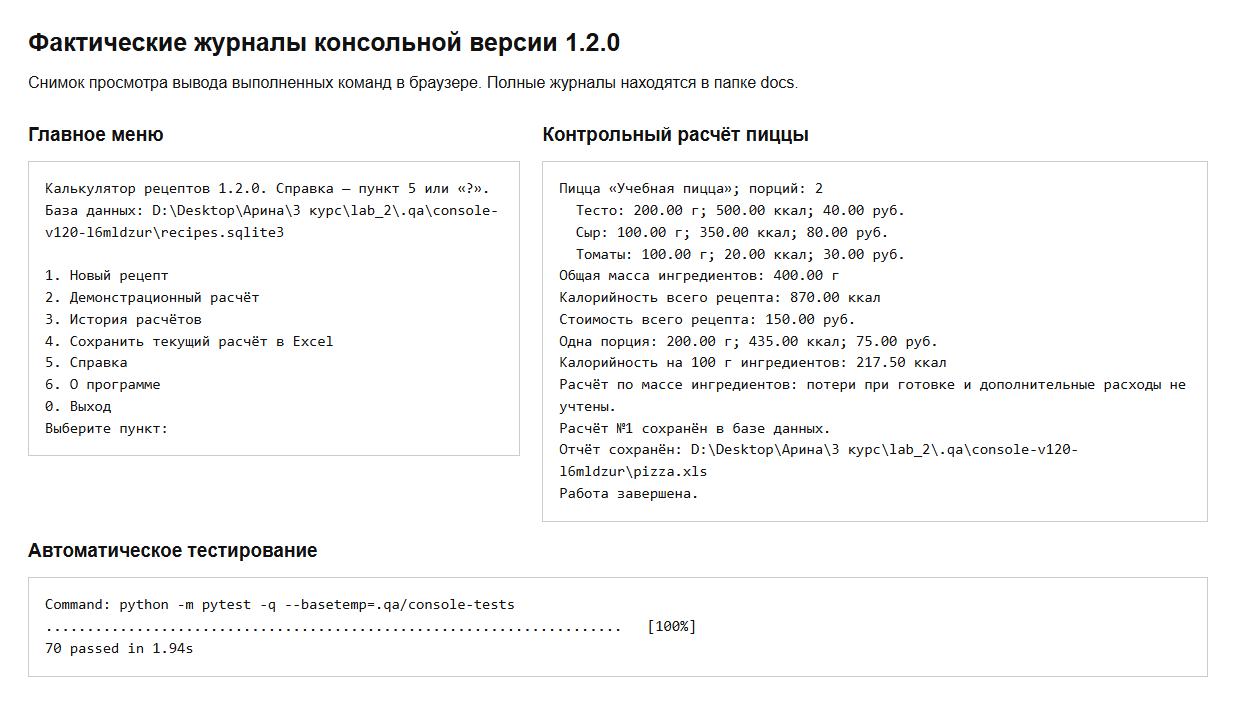
\includegraphics[width=\textwidth]{evidence/console-evidence.png}
\caption{Просмотр фактических журналов меню, контрольного расчёта и pytest в браузере}
\end{figure}
Полные журналы сохранены в папке docs проекта. Фактический итог: 70 тестов пройдены.

\subsection{Docker}
Проверка выполнена 17 ноября 2026 года: Docker Desktop 4.99.0,
Docker Engine 29.9.3 (Linux/amd64), Compose 5.7.0.
Конфигурация Compose прошла проверку, образ recipes-lab:local собран.
Dockerfile устанавливает зависимости до запуска приложения.
Локально и в контейнере используется единый консольный интерфейс main.py.

Первый контейнер рассчитал пиццу: 870 ккал, 150 руб., создал SQLite и Excel.
После его удаления второй контейнер прочитал те же файлы и проверил результат.
Это подтверждает сохранность данных между контейнерами.
Также проверены меню без аргументов, справка, раздел <<О программе>> и выход через Compose.
В образе отсутствуют графические библиотеки.

Итог verify\_docker.py --- PASS. Полный журнал:
\texttt{docs/docker-verification.txt}.
Тестовые контейнеры удалены с --rm; образ и данные сохранены.
Требования Well-done по SQLite и контейнерному запуску подтверждены.

\section{Вывод}
Разработан калькулятор калорийности и стоимости вока, бургера и пиццы.
Приложение имеет модульную структуру, объектную модель,
проверку управляемых атрибутов, справку и историю.
Результат сохраняется в SQLite и Excel.
Предметные расчёты и основные сценарии проверены тестами pytest.

\section{Использованные материалы}
\begin{enumerate}
\item Методические указания algorythms\_python\_lab\_02.docx.
\item Python ABC: \url{https://docs.python.org/3/library/abc.html}.
\item Python Decimal: \url{https://docs.python.org/3/library/decimal.html}.
\item Python SQLite: \url{https://docs.python.org/3/library/sqlite3.html}.
\item xlwt: \url{https://xlwt.readthedocs.io/en/latest/api.html}.
\item pytest: \url{https://docs.pytest.org/en/stable/}.
\item Dockerfile: \url{https://docs.docker.com/reference/dockerfile/}.
\end{enumerate}
Формулы получены пересчётом с базы 100 г на фактическую массу и
сложением вкладов ингредиентов; пищевые справочники не использовались.

\clearpage
\appendix
\section{Листинг программы}
\subsection{Основная программа}
\VerbatimInput[fontsize=\tiny]{listings/main.py}
\subsection{Модель и расчёты}
\VerbatimInput[fontsize=\tiny]{listings/models.py}
\subsection{Сохранение SQLite}
\VerbatimInput[fontsize=\tiny]{listings/storage.py}
\subsection{Вывод и экспорт}
\VerbatimInput[fontsize=\tiny]{listings/reports.py}
\subsection{Инициализация пакета}
\VerbatimInput[fontsize=\tiny]{listings/__init__.py}
\subsection{Dockerfile}
\VerbatimInput[fontsize=\tiny]{listings/Dockerfile}
\subsection{Compose}
\VerbatimInput[fontsize=\tiny]{listings/compose.yaml}
\subsection{Проверка контейнеров}
\VerbatimInput[fontsize=\tiny]{listings/verify_docker.py}
\end{document}
